\title{Hierarchical temporal framework for reinforcement learning: an end-to-end model of the brain}
\author{Aleksander Mendoza}
\newif \ifanswers

\documentclass[12pt]{article}
\usepackage{tikz}
\usepackage[utf8]{inputenc}
\usepackage[T1]{fontenc}
\usepackage{lmodern}
\usepackage{amsfonts}
\usepackage{mathrsfs}
\usepackage{centernot}
\usepackage{listings}
\usepackage{mathtools}
\usepackage{xcolor}
\usepackage{amsthm}
\usepackage{amsmath}
\usepackage{amssymb}
\usepackage{tikzit}
\input{style.tikzstyles}

\newtheorem{definition}{Definition}
\newtheorem{theorem}{Theorem}[section]
\newtheorem{corollary}{Corollary}[theorem]
\newtheorem{lemma}[theorem]{Lemma}
\renewcommand{\labelenumii}{\theenumii}
\renewcommand{\theenumii}{\theenumi.\arabic{enumii}.}
\begin{document}
\maketitle
\lstset{
	basicstyle=\ttfamily,
	mathescape
}

\begin{abstract}
	Over the recent decades neuroscience has created many theories explaining the functioning of each part of the brain in separation but a general unified theory of the brain was
	still lacking. Meanwhile in the field of artificial intelligence, reinforcement learning has been struggling with its own problems of sample efficiency
	and catastrophic forgetting. This paper draws parallels between neuroscience and reinforcement learning and provides a unified theory of the brain
	that combines the two fields and solves their respective problems. It provides a new way of looking at reward and shows what mechanisms are necessary to achieve one-shot reinforcement learning, analogical to that observed in humans and animals. It explains in detail the mechanisms responsible for emergence of place cells in the hippocampus, voting in the neocortex, pattern separation and lamellar structure of dentate gyrus. It gives some outlook for the near future of this new architecture
	and the first blueprint for achieving general human-like AI capable of abstract thinking.
\end{abstract}

\section{New perspective on reinforcement learning}


Over the recent years, the dominant paradigm for building intelligent agents has been that of deep reinforcement learning. Its origins stem from control theory and Markov decision processes. This model of learning treats interactions with the environment as a tree of all possible decisions. Every state of the world is a node in that tree and each action taken by the agent is an edge connecting two nodes. It's a simple idea and mathematically beautiful abstraction over the real world, because it reduced the complex issue of control and interaction into the problem of traversing a tree in hope of finding the path with largest total value (known as reward). It is important not to forget that all abstract models are wrong, but some of them are useful. The control theory was
of great importance to deep reinforcement learning, as it allowed treating the interactive environment as yet another function to be approximated. This was the perfect task for deep neural networks. Thanks to the geometric theory of deep learning, today we know with greater detail how powerful deep neural networks are for finding function approximations.

While data-driven problems such as computer vision, natural language processing and speech recognition are to a large extent `solved', the issue of control and decision-making has so far seemed to be fundamentally different. Over time it became apparent that deep reinforcement learning has serious shortcomings. While in all other modalities transfer learning is widely adopted, it remains a challenge here. Once a certain control task is mastered, fine-tuning the same network for another usually leads to catastrophic forgetting. The process of training itself is also problematic. The convergence is highly sensitive to initial conditions and random exploration. Sample inefficiency renders our current methods unsuitable for most practical applications. All the great achievements of deep reinforcement learning that generated media headlines, have only been possible at the cost of immense computational power, accessible only to a few large corporations. 

Meanwhile our biological brains can adapt to new environments nearly instantaneously and quickly assimilate new information, without forgetting the previously learned facts. Some may say that the real brain is much larger than any artificial neural network built so far and reaching human-level intelligence is merely a matter of scale. This argument largely falls apart when we put into perspective the fact that training large language models often consumes as much electricity as entire cities, whereas biological brains use only the power equivalent of a lightbulb. Artificial networks have millions of layers, real brains only a handful.
ResNet already scores higher on image-recoginition tasks than humans and yet does not understand the data it sees. This casts a doubt over the validity and relevance of our existing approaches and abstract models. The next step in developing reinforcement learning  does not need larger and more sophisticated networks. A paradigm shift is crucial and it will likely give us far simpler and more efficient architectures. Control theory and Markov decision processes are not the right abstraction and they only lead our research towards a deceptive local optimum of scientific results. The reward is not enough. This paper strives to provide an alternative.

The fundamental building block of control theory is a decision. All interactions with the world are represented as decisions about consecutive  actions taken by the agent. The theory of Markov decision processes solves control tasks by ranking the possible actions and then greedily making the best decisions. We would like to argue for a different perspective. Our fundamental building blocks are locations on a map. Learning is not the matter of finding policy or ranking actions, but rather it's about uncovering this latent map. Once it's uncovered, the agent can know, which direction to go and which actions will lead there. Inside our brains there is no policy function. Instead we have an internal map in the hippocampus. It is not a two dimensional Cartesian map, but rather a high-dimensional manifold of abstract ideas. It does not encode position using scalar coordinates. Instead it encodes both space and time using populations of neurons. Deep reinforcement learning builds such maps in an inefficient roundabout way with the policy gradient. Our brains use much more efficient episodic memory algorithm. In deep learning, exploration is implemented by taking random actions with epsilon probability. Such approach is naive and inefficient. Instead, by having an internal map and memory of past events we can  always precisely tell which areas are known and which remain to be explored. Once we undertake a new path, we record the experience onto our internal map. This mechanism effectively allows  for one-shot reinforcement learning, similarly to the way it has been observed in humans and animals. In the real world, organisms must make optimal use of their energy. Taking a shorter path is more optimal, because walking and running is expensive. Organisms are rewarded for finding food, which is a source of vital energy, whereas redundant activity is discouraged. This definition of reward solves the problem of exploration. An agent should explore new environment if it has either abundant reserves of energy and can afford to freely forage or all the previously known energy sources have run out and new need to be discovered.
In artificial settings the energy could be programmed to encourage certain specific desired outcome. So far the field of reinforcement learning has been obsessively focused on `reward' but here we argue that in fact it's better to think in terms of `hunger'. Then the `reward signal' becomes nothing more than a special case of `hunger signal'. Instead of  `reward shaping', which is difficult and error-prone, it should be easier and more natural to program agents by `hunger shaping'. Reward is received when hunger decreases.

The field of reinforcement learning stands to benefit a lot from changing  its perspective. We should stop thinking of decisions and start framing all problems as spacial navigation tasks. Perhaps it is not a coincidence that in the early days, most original examples, thought-experiments and challenges were based on path-finding problems (Figure \ref{fig:rl_problems}).

\begin{figure}[!htbp]
	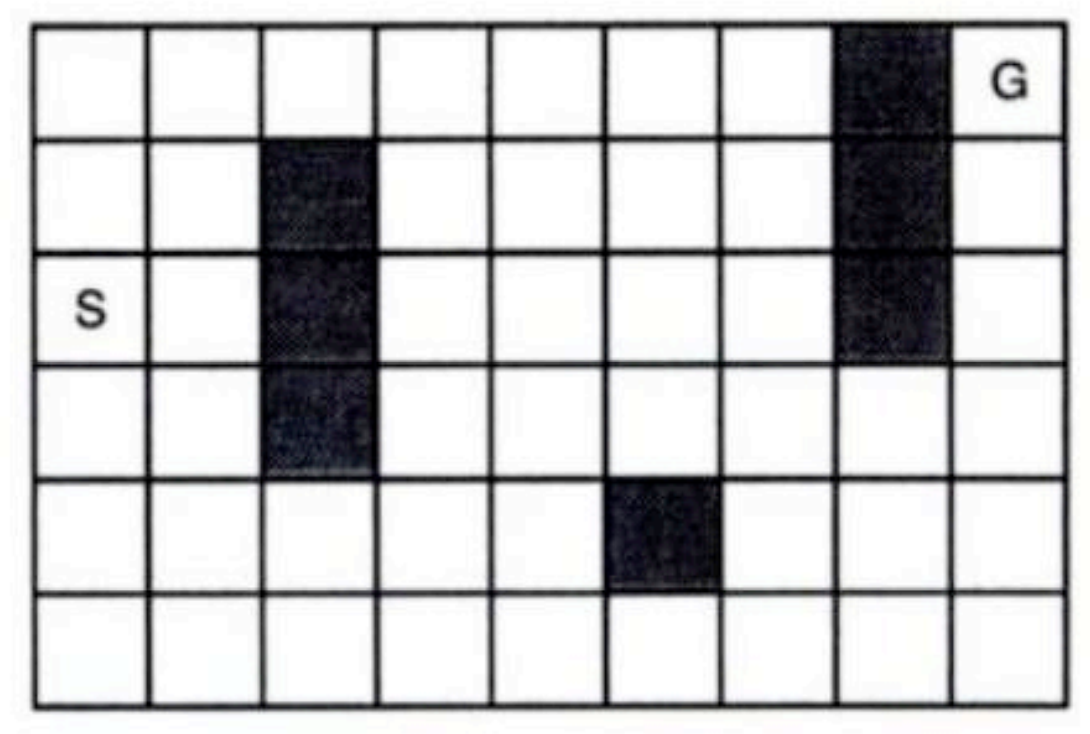
\includegraphics[width=7cm]{dyna}
	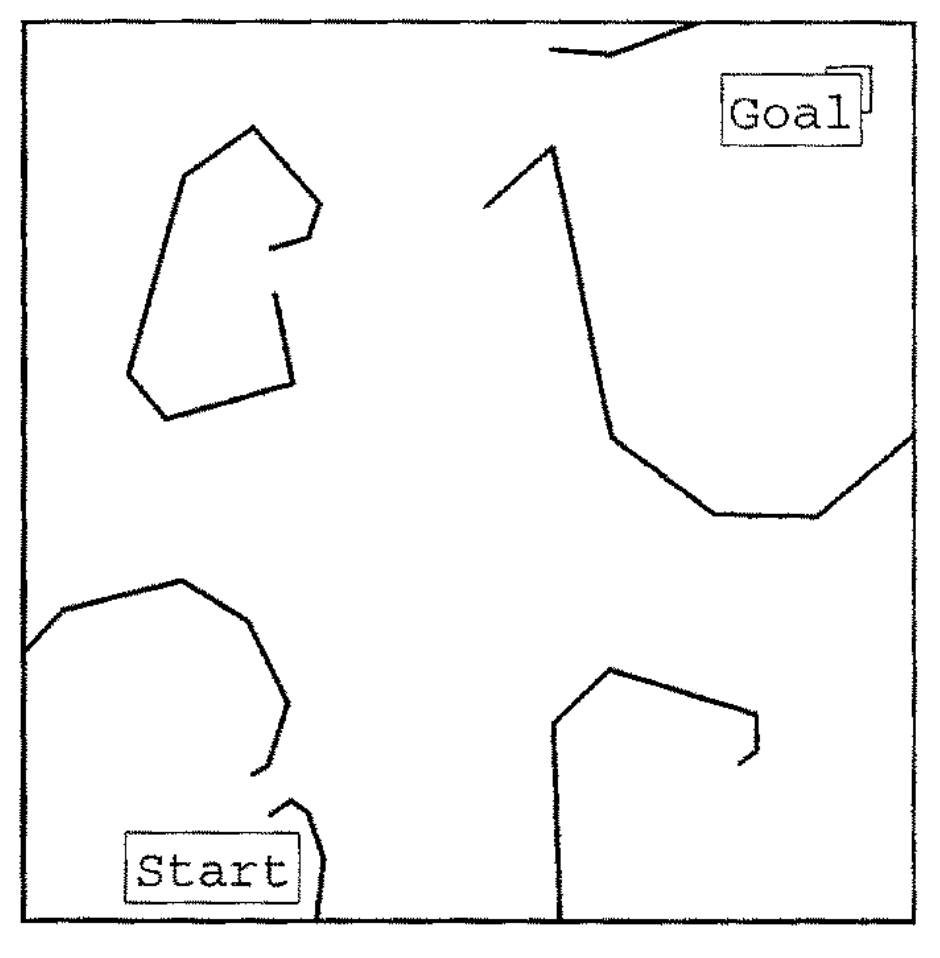
\includegraphics[width=7cm]{parti_game}
	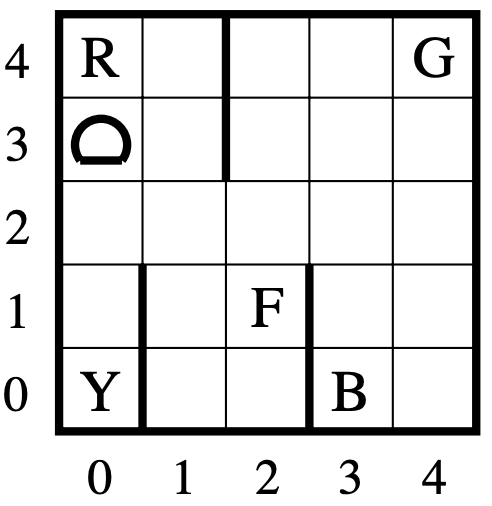
\includegraphics[width=8cm]{maxq}
	\caption{Navigation has always played a central role in reinforcement learning problems. Examples found in Sutton 1990 \cite{dyna} (upper left), Moore and Atkeson 1995 \cite{parti_game} (upper right), Dietterich 1998 \cite{maxq} (bottom) }
	\label{fig:rl_problems}
\end{figure}


The spacial navigation task seemingly appears to be a special case application of policy gradient. We want to argue that it's the opposite, although for a long time it was not trivial to spot how every reinforcement learning problem could be reduced to a map navigation. The general intelligence of humans works thanks to such abstract maps of ideas. When we attempt to solve a mathematical problem we are searching through our internal map of mathematics. That's the reason why a new math problem at school may seem difficult the first time we encounter it, but if we solve it once, then we add a new path to our internal map and we use the same path to solve all other similar tasks. The first time we attempt to pay our taxes we may struggle and we might now know where to start, but every subsequent time is easier, once we saw the general procedure. This pattern of learning can be applied to almost every other skill. This is the definition of general intelligence.

We provide an end-to-end  machine learning architecture capable of  building such abstract manifold maps. Before we present it some additional background is necessary. Deep learning is a tool for function approximation. Maps are not functions (even though deep reinforcement learning has been desperately trying to pretend that they are). Hence this cannot be achieved with the familiar methods. Instead, maps are built by associations. The right tool to for this task are Hierarchical Temporal Memory networks.

\section{Hierarchical Temporal Memory} 

Our architecture is primarily based on HTM networks, although we add two new important mechanisms. Those are pattern separation and voting. 

Pattern separation is a property of dentate gyrus, which takes as input very similar patterns and produces new output with much less overlap among the neuronal populations. In reinforcement learning this feature could allow the agent to differentiate between similar situations. For example eating most frogs might be safe but those with red stripes under their eyes might be poisonous and should be avoided. Figure \ref{fig:pattern_sep} presents a graphical illustration of this phenomenon. 


\begin{figure}[!htbp]
	\centering
	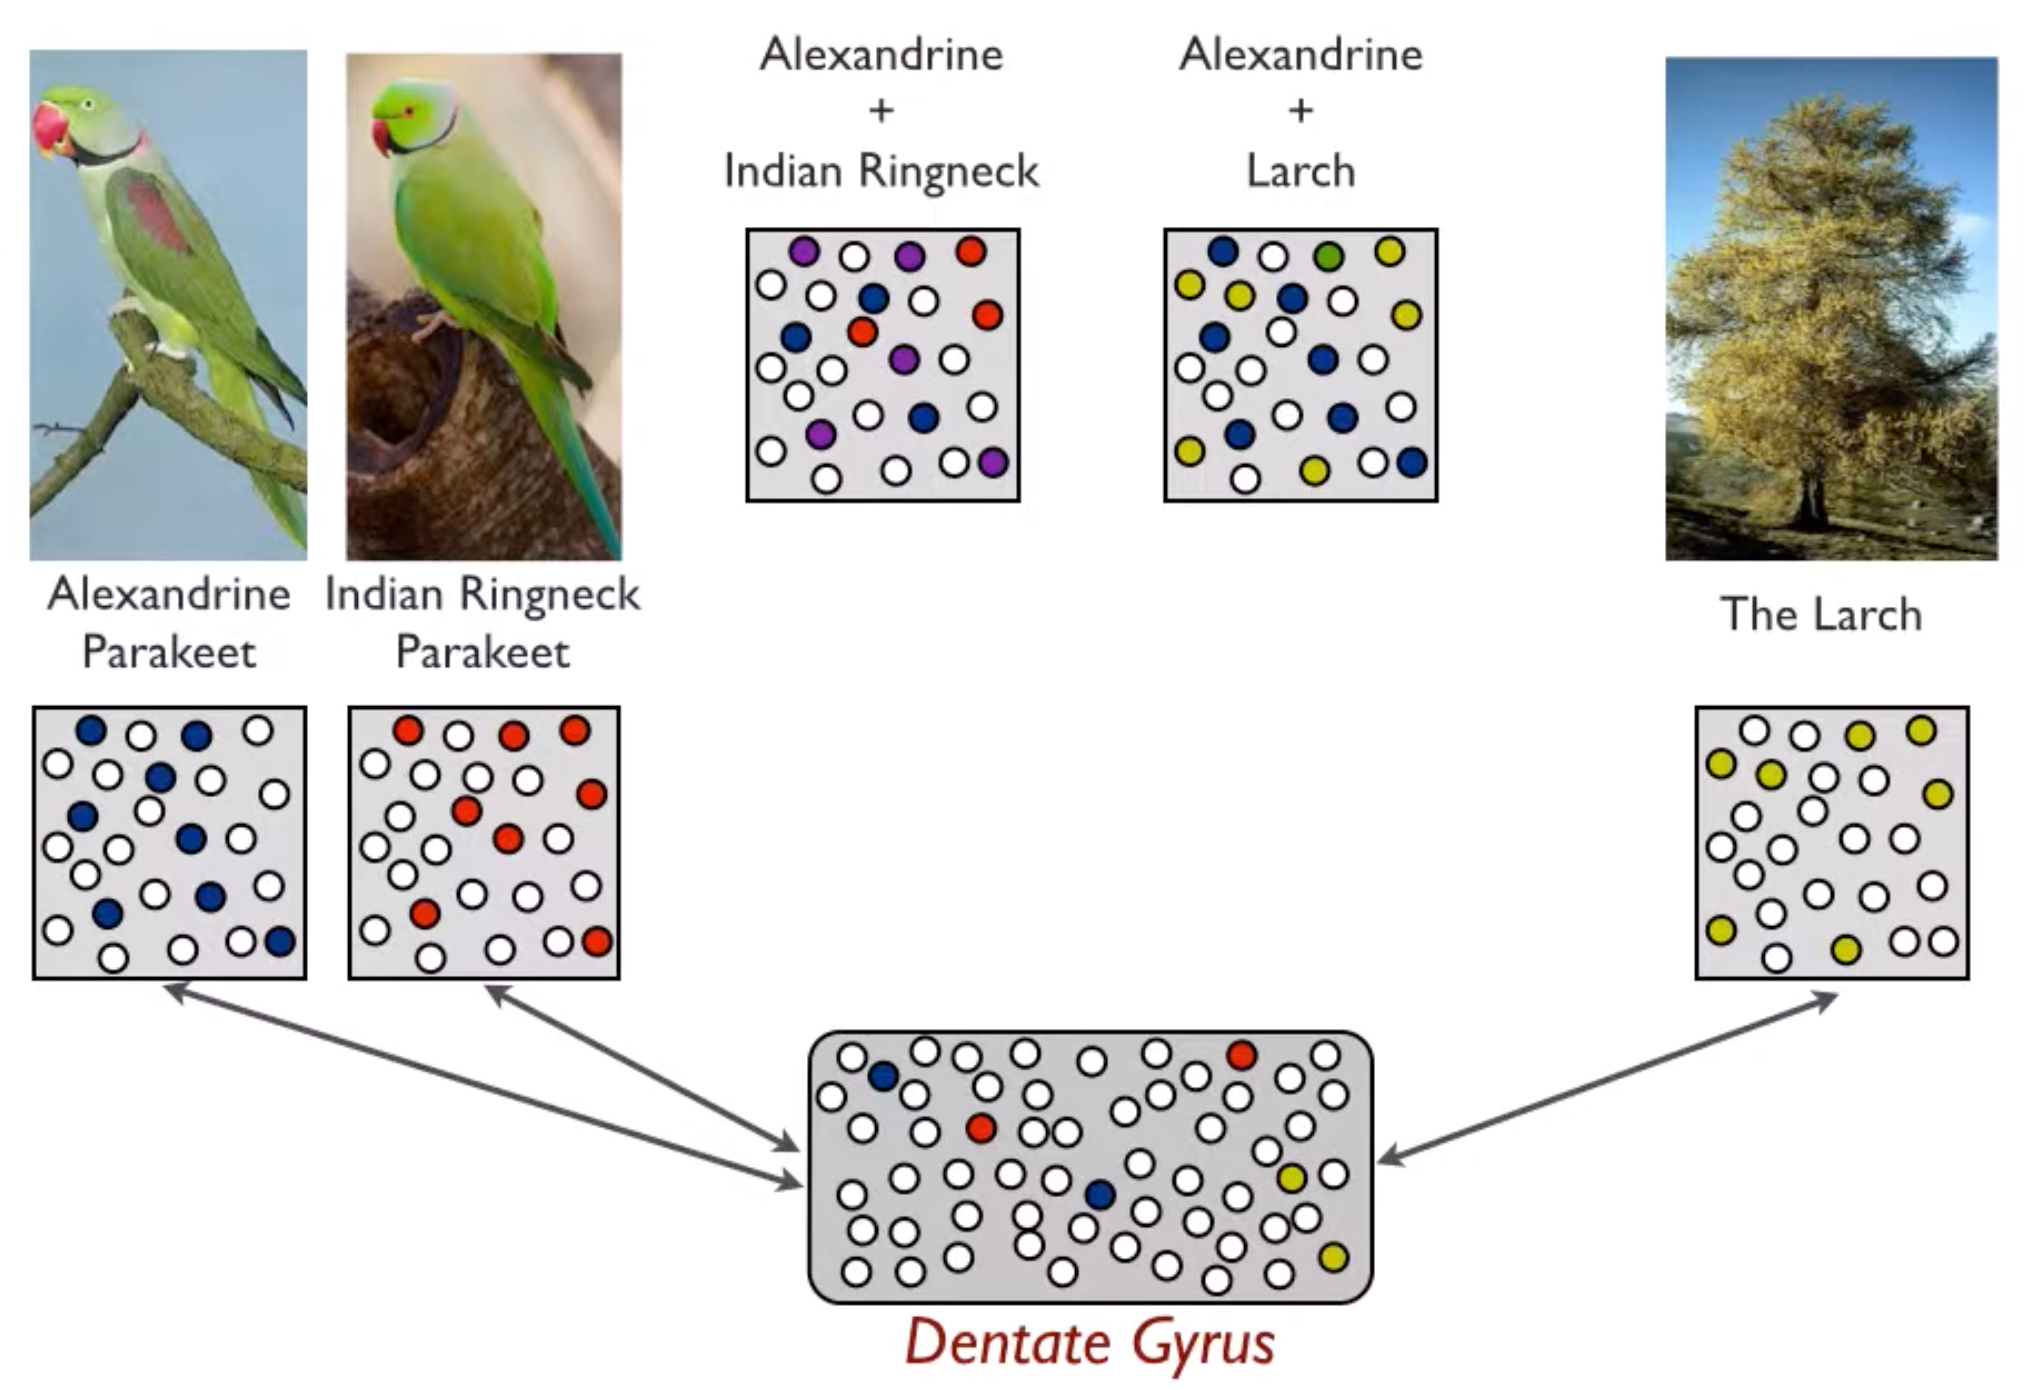
\includegraphics[width=10cm]{pattern_sep}
	\caption{A bird and a tree are easy to tell apart and their internal representation in the network will likely produce non-overlapping activation patterns. Finding a difference between different similar species is a greater challenge. A typical neural network would need to be specifically trained to produce distinct embeddings, but our brains use dentate gyrus to solve this problem much more efficiently. Graphics from \cite{pattern_sep}.}
	\label{fig:pattern_sep}
\end{figure}

The effects of pattern separation are measured as the average overlap in pairs of input and output patterns. It can be reproduced by spacial pooler if the learning is disabled (increment and decrement constants are zero) and the size of output layer is increased. Figure \ref{fig:dg_pattern_sep} compares experimental results in biological brain and in a simulated HTM network.



 \begin{figure}[!htbp]
 	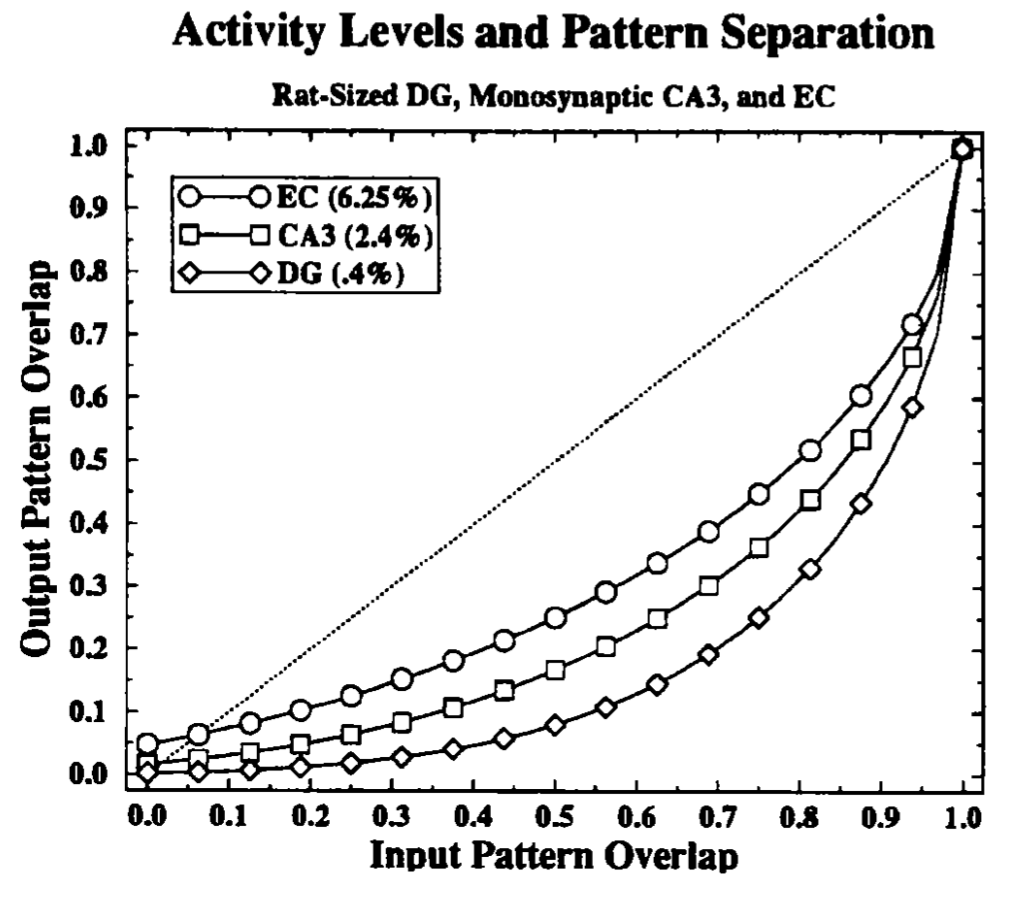
\includegraphics[width=7cm]{dg_pattern_sep}
   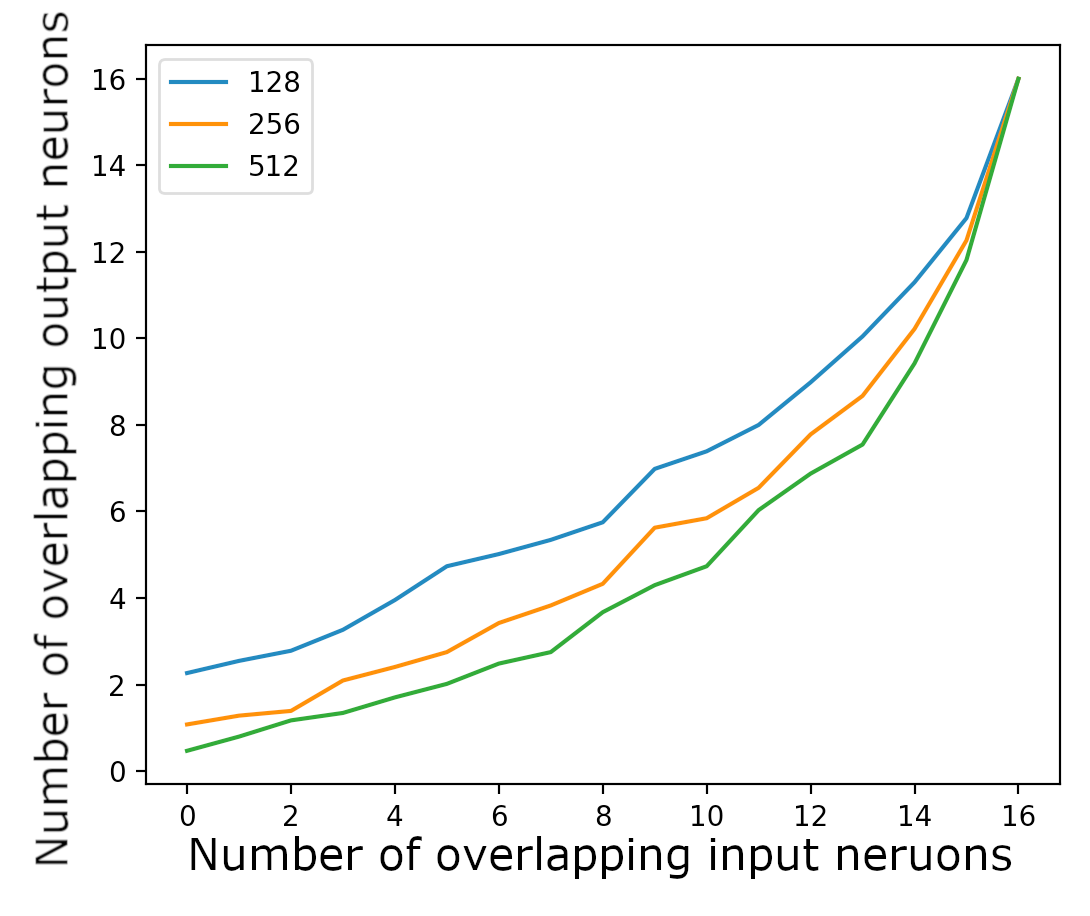
\includegraphics[width=7cm]{exp_pattern_sep}
 	\caption{Left: Empirical approximation of the effects of pattern separation in dentate gyrus (DG), entorhinal cortex (EC) and hippocampal area CA3. Data taken from \cite{dg_pattern_sep}. Right: Experimental benchmarks of pattern separation in spacial pooler with input layer of size 128 and output layer of respective sizes 128, 256 and 512. In these experiments random populations of 16 input neurons were generated. Spacial pooler's sparsity has been configured to always choose 16 most active output neurons.}
 	\label{fig:dg_pattern_sep}
 \end{figure}


Another property crucial for understanding our architecture is voting. In the standard deep learning setting, a network will receive some inputs and then have softmax output layer that classifies  the data and assigns some label. A spacial pooler could be used in an analogical way. Labels could be encoded as categorical data (subdivide a network into $n$ parts, one for each label and then activate neurons in only one part corresponding to the current label). The input receives some sparsely encoded data and spacial pooler will activate some output population of neurons. To determine the prediction made by network, choose the label that has the largest overlap with currently active output (this is analogical to softmax function). In order to learn the labels, it is enough to increment connections to those active neurons that did overlap with the correct label. In the biological networks it would be equivalent to apical feedback (the correct label) partially depolarizing the output cell. 

The above supervised learning example was simple but consider what happens in the case of unsupervised learning. This means that instead of modelling probability $P(label|input)$, we build a network that sees both label and input. The we is asked it to model joint probability $P(label, input)$. This scenario also has an analogy in HTM networks. This time we have two columns, each one receiving different input. The first one might see
patch of pixels, a range of audio frequencies, a few scalar values or any other piece of information. The other column might have access to the label. We could then add distal connections from output of first column to output of the other and use patterns produced by one to predict the other. First compute output of column A, then use distal connections from A to B in order to activate B. Next compute output of B based on its input and compare with the activity anticipated by distal connections. Such process could be repeated for both columns and train one from the other in an unsupervised way. This could be generalised further and both columns could be reading different inputs, rather than labels but the fundamental idea is to use activation patterns of different columns as if they were labels.

It is possible to combine both supervised and unsupervised methods into one. There could be distal input coming from neighbouring columns and apical input from above. The most unintuitive and difficult problem is how to generate the apical feedback. We propose an interesting solution. The key insight is that our brains evolved in an environment that is time-consistent. When the observed inputs evolve slowly over time, then if we use activity patterns from previous time step we have high probability of still being correct and up-to-date. What's what we call `sticky' layers. We could compute activations of higher columns once and then use them as apical input in all subsequent steps until something significant happens that forces the higher columns to update. If we have multiple lower columns all connected to the same higher column, then we could put threshold on how many lower columns must agree together in order to overwrite a higher column in case of disagreement. Until there is enough consensus in lower parts, the higher levels do not change. If nobody agrees with anyone and the consensus threshold is not reached, then the higher layers take precedence and their activity is used as labels for the lower ones.
Lastly it should be noted that the higher columns can be initialized randomly at the beginning. If the environment is time-consistent then the system will always settle on some consensus in a self-organizing manner after enough time steps.


\section{End-to-end model}
The architecture is inspired by the biological brain, albeit much smaller and more simplified. The most significant novelty is that it is the first end-to-end model of the brain.  It consists of 3 layers and a map unit. Those layers are vaguely related to their respective biological equivalents.
This correspondence should be taken with a grain of salt, as the goal of this architecture is not to focus on any specific biological brain, but rather to identify the universal mechanisms underlying all key functions. It should be expected that this model is one of many possible architectures and future research will explore more alternatives, regardless of how similar they are to the real brain.
 
\ctikzfig{architecture}

The sensory inputs come from many modalities like vision, hearing or touch. This part of the network is typically either evolved using population-based algorithms or designed manually. It might also be possible to substitute it with deep neural networks trained with backpropagation, although this area requires more research. 

The input arrives at the first layer, which was primarily inspired by the neocortex. It consists of one large spacial pooler. It's task is to extract key information from the input and prepare it for voting in the next layer.

The second layer is another spacial pooler whose task is to build representation of agent's immediate surroundings. It has been largely inspired by the Entorhinal Cortex, which contains grid cells, head-direction cells and other spacial features. We argue that the grid cells themselves are not necessary and this model does not include them. The visual, auditory and olfactory cues are sufficient and crucial for building map of surroundings. We suspect that grid cells are only an addition that allows for greater precision of navigation in the absence of cues (for example in a dark room or water maze experiments). The neurons of second layer encode features on a sphere (Figure \ref{fig:rodent_in_sphere}). 


\begin{figure}[!h]
	\centering
	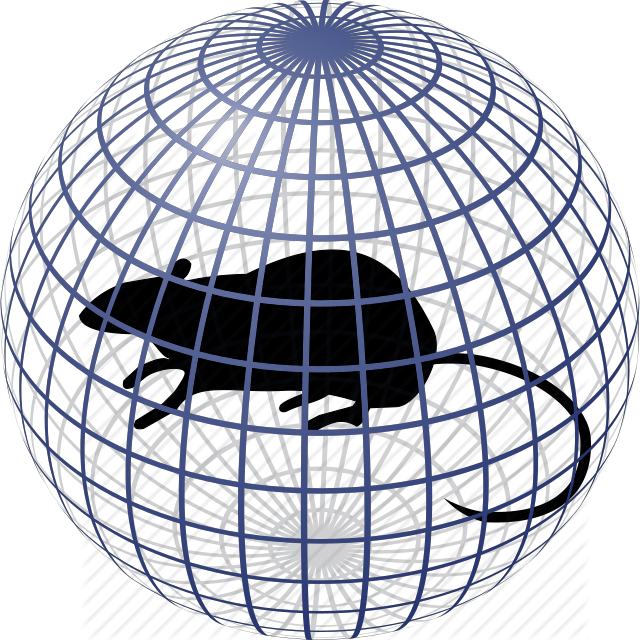
\includegraphics[width=7cm]{rodent_in_sphere}
	\caption{The second layer is topologically equivalent to a sphere surrounding the agent. Each point on its surface contains information about distance and label of a visible object. Hence it forms both a depth-map and outlines of all objects.}
	\label{fig:rodent_in_sphere}
\end{figure}

The sensory input that is received by the network contains information about distance. This is the reason why all animals have two eyes and two ears. By comparing the view from one eye with the other or the sound delay in one ear against the other, they receive information about position in space (some, like birds, don't have stereoscopic and they bob their heads instead). This information is crucial and must be preserved by the networks processing the sensory inputs.  The first layer (neocortex) will build internal representations of objects at their respective locations. Then all perception will be mapped onto the sphere and locations that end up close to each other on the sphere will clash (there might be less storage capacity on the sphere than there is in the layer 1). In order to resolve these clashes, some voting mechanism is necessary. This voting occurs not only across space but also time. The labels attached to each location are `sticky'. The network has many attractor states and in order to change the label, there must be enough signal coming from outside to knock the network out of its current stationary point. This is a useful property because the real environment tends to be consistent across time. Usually most objects don't move and when they do, the location at next time step is close to the location from previous one. Hence we can use labels from last time step to train layer 1 in the next step. This introduces an (apical) feedback input from layer 2 to 1.
This mechanism of time-delayed self-training is very common and we will also use it again later to train the map.
Because the labels are `sticky', they will remain intact when the agent looks in another direction. Hence it will be aware that the objects do not disappear and are still there even though they are not visible. The sphere itself is the simplest geometrical object that is sufficient to make the layer 2 work, although in biological networks it might be a more irregular shape. The depth-map on a sphere is not well suited to represent concave environments. Modifications to the current mechanism will likely be explored in the future, but the current one is the simplest that suffices. 

Layer 3 exhibits the least plasticity and does learn any internal model itself. Its sole task is to facilitate pattern separation. It is much larger than the previous layers. In biological brains it corresponds to dentate gyrus, which is known for being the area most densely populated with neurons. It is implemented as a spacial pooler with low or zero plasticity and a significantly sparser activation. It receives input about the immediate environment and turns it into unique fingerprints that will later be used as the basis for episodic memory.  The connections between layer 2 and 3 have a special property of invariance but in order to explain it, we must first go back to layer 1. As the agent moves its head around the locations of features must rotate along with it, but the output of layer 3 should remain rotation invariant. This could be better explained with a simplified example in two dimensions, using circle instead of a sphere (Figure \ref{fig:rodent_in_circle}). 

\begin{figure}[!h]
	\centering
	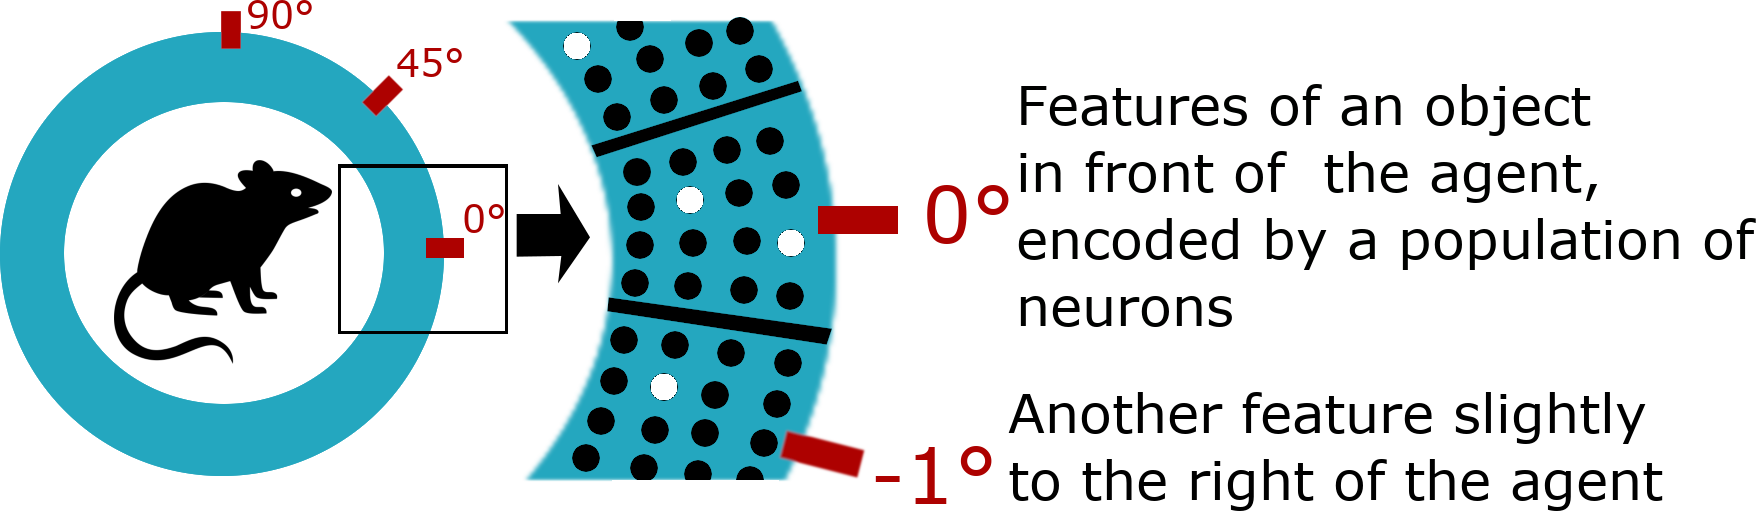
\includegraphics[width=11cm]{rodent_in_cirle}
	\caption{Layer 3 topologically equivalent to a circle contains features of objects in the immediate environment of the agent}
	\label{fig:rodent_in_circle}
\end{figure}

The circle is subdivided into segments containing neuronal populations. Each one of them encodes features of some object visible to the agent at a different angle. Those angles are defined relative to agent's head direction. It is necessary, because the inputs incoming from layer 1 are all  defined relative to the head. The information where objects are located is not encoded by neuronal populations but rather by the topology of connectivity patterns in sensory networks as well as layer 1. Our model makes one simplification and assumes that eyes cannot move freely, but rather the view angle depends solely on head position. Hence a specific neuron of layer 1 will fine only if a feature has been detected at a specific angle relative to the head. As the agent rotates its head, the `sticky' populations on the sphere of layer 2 could become misaligned with subsequent inputs from layer 1. In order to ensure that the internal representation does not become detached from the real world, this model will use feedback from motor units to decide when to shift its neuronal populations on the sphere. For example if the agent decides to move its head 1° to the right, then the activity pattern at current -1° population will move to  0°. Pattern from  0° will move to  1° and so on. The important part is that the agent already anticipates the rotation even before motor units perform the desired movement. Then in the next time step the motor movement will be executed and layer 1 will contain information about cues at slightly shifted locations. If the sphere of layer 2 performs its rotation correctly, then the new input from cues in layer 1 will be perfectly aligned with anticipated activity pattern in layer 2. We could argue that the effects of this mechanism could also be experienced in the real brains. For example when we are scrolling through internet pages on a computer screen we already anticipate that the text will move upwards. If for some reason it doesn't (battery in the mouse suddenly runs out) we experience the relatable feeling of misalignment, caused by layer 1 not agreeing with anticipated locations at layer 2. Another example might be the dizziness experienced after spinning on a rotating chair. Even after we stop spinning, our brains already learned (possibly by plasticity in attractor networks that might implement biological mechanisms of layer 2) to anticipate constant rotation and now a short period of time is needed to unlearn this behaviour.

The mechanism above described why the sphere needs to rotate and how to implement connections between layer 1 and 2. The final step in building a model of immediate environment is to design connections between layer 2 and 3 in such a way that makes them rotation invariant. This could be achieved by repeating the same connection pattern for all possible angles (Figure \ref{fig:rotation_invariant_pattern}). 

\begin{figure}[!h]
	\centering
	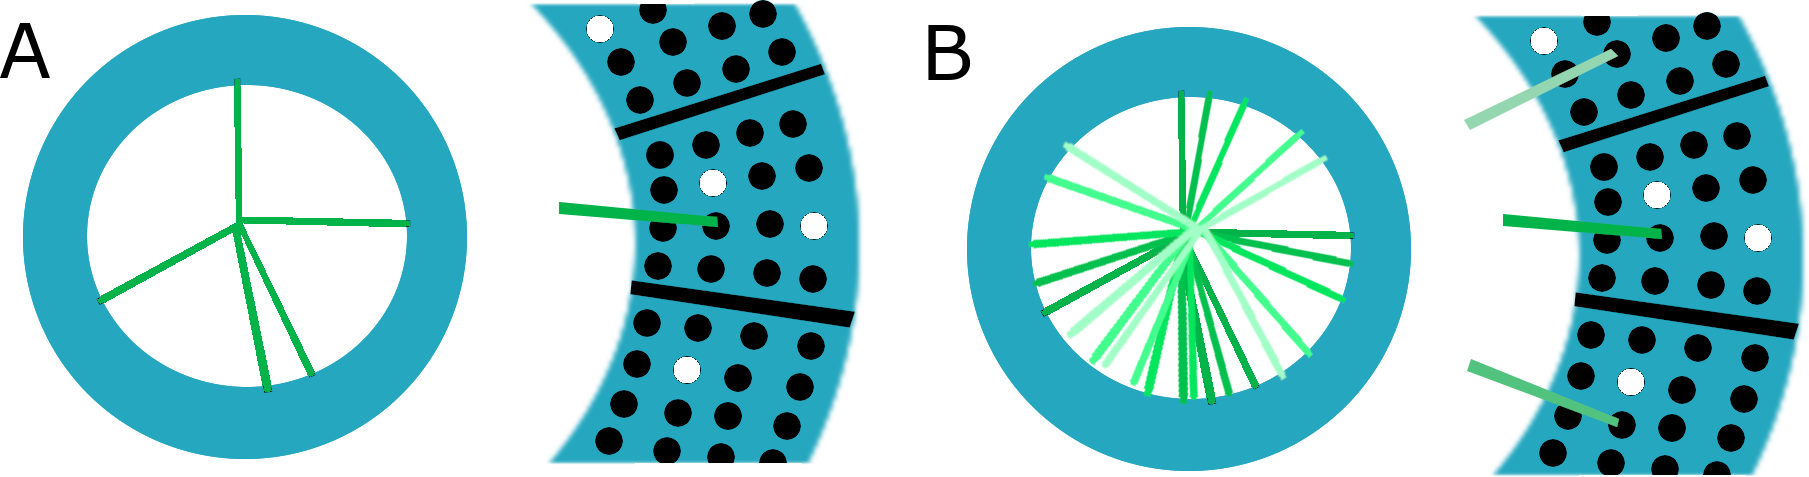
\includegraphics[width=11cm]{rotation_invariant_pattern}
	\caption{Left: a single dendritic segment implementing some connectivity pattern. Right:
	 the same segment repeated for each rotation. The postsynaptic cell will fire if any of the
    segments recognizes the pattern.}
	\label{fig:rotation_invariant_pattern}
\end{figure}


In HTM networks it is implemented by repeating the same dendritic segment for each rotation. If the connections were plastic, then there would be a risk that over time the segments would rewire themselves and diverge from the original pattern. What a coincidence that pattern separation works best when plasticity is disabled. It also has some 
analogies to biological brains. Dentate gyrus has highly organized lamellar structure, suggesting that regularity of connections might be crucial and could facilitate implementation of mechanisms similar to our model. Even if it turned out that layer 2 is not a sphere but rather a more complex shape, dentate gyrus might express various invariant properties in those different geometries. It should be stressed that regardless of how biological our model might be, the invariance mechanisms used by us were mostly driven by necessity rather than any explicit attempt at being biologically plausible. 


The final and most important component of this model is the map. Similarly to layer 2, the neuronal activations here are also sticky. A population of active neurons does not change no matter what input comes from layer 3. The only possible way to update the activity pattern in the map is when the agent changes location in the environment. Until this happens, the currently active neurons are used as `labels' for training connections between layer 3 and the map. Each time a new observation of the environment comes in, passes through layer 2 and causes some new activity in layer 3, we associate that new activity with currently active cells in the map and strengthen the connections between them. The plasticity is modulated by currently received reward. If the agent found source of energy that decreased its hunger, the reward will be high and the plasticity will be much stronger. When the agent decides that it's time to move and changes its location, the map will change its activity pattern. Within the map itself there are also many recurrent contextual connections. Their implementation is similar to the temporal memory algorithm in HTM networks, but there is one difference. There are several types of distal segments, one for each action and one additional for time compressed sequence of actions. Those connections encode information about the actions taken by the agent as it navigates through the environment. The time agent finds itself in the same spot it will be able to imagine and plan future trajectories by following those strengthened recurrent connections. The plasticity again depends on reward.
When an agent stops at point $X_0$, then takes actions $a_1, a_1, a_2... a_n$ to traverse through locations $X_1, X_2, X_3,...X_n$ and the finally stops as location $X_n$, the path of recurrent connections corresponding to transitions  $(X_0,a_1)\rightarrow X_1$, $(X_1,a_2)\rightarrow X_2$ ... and so on, will be strengthened. Depending on whether $X_n$ contained a reward or not, the plasticity will be different but some strengthening will always take place. For a single trajectory, it is necessary to perform the strengthening in several iterations. As long as the agent remains idle at state $X_n$, the map will keep replaying the last trajectory and strengthening it. With each subsequent replay, it will omit certain intermediate steps. This allows for the effect called time compression. As a result, next time agent finds itself in the same spot $X_0$, it will be able to plan future trajectories in stepping stones, rather than individually  action by action. This allows agent's imagination to efficiently make plans running far into the future. The stepping stones usually will be the idle states like $X_0$ or $X_n$ and the intermediate states will slowly fade out of the memory over time. If the agent then decides to continue walking and reaches  a third idle state $X_m$, then during planning the agent will hop through sequence $X_0\rightarrow X_n \rightarrow X_m$. During execution of the plan, the agent will find itself first at state $X_0$ and its goal will be to reach $X_n$, however there will be no state-action pair in its memory corresponding to $(X_0, a)\rightarrow X_1$. Instead there will be a memory of $(X_0,a_1)\rightarrow X_2$ and this will be chosen. If over time it turns out that the agent frequently traverses trajectory $X_0...X_n...X_m$, it might start forming a routine. It will less often stop at $X_n$. Instead most of the time it will start executing trajectory $X_n...X_m$ immediately. As a result, no stops will be made at $X_n$ and it will slowly fade out of memory as well. In the end the agent will only remember  the stepping stones $X_0...X_m$. This is the mechanism by which the less important stepping stones are dropped from the memory and only the important fragments of each episode are retained. Biologically this mechanism corresponds to the episodic memory of hippocampus. The neurons active in the map correspond to place cells, which fire only when animal finds itself in a specific location. For a long time neuroscience was not able to explain the exact mechanisms responsible for formation of place cells. This paper is the first one to give this explanation in form of a precise algorithm. Our model is biologically plausible, except only for segments encoding actions (in reality there might be additional neuronal populations coming from motor feedback, but our model simplifies it and works with a manually programmed set of actions instead). It has been observed that the brain activity of idle animals
is very different from the actively moving ones. During idle states, hippocampus often experiences sharp-wave-ripple events, which replay the recent experience in reverse order. Our model does not require to perform the replay in reverse. It might be a necessary mechanism for biological neurons, but a computer algorithm might as well temporarily store the sequence of actions in a data structure. We suspect this should not make a significant difference. Another parallel that could be drawn is the reward system. In biology, the brain will secrete dopamine, which serves the same purpose, but in virtual environment the hunger-reward system might be either programmed by hand or fine tuned using evolutionary methods.  

Lastly our model leaves room for feedback connections from the map to layer 1. This allows for recall of past memories and reliving their experiences. It can be trained in the same way as the connections between the map and layer 3. The real brain uses attention mechanisms to only focus on certain important fragments of the experience, instead of making perfect recordings of the past like a movie. We do not include such mechanisms in order to keep the model simple. Analogically not all actions are equally important. An agent being in an idle state is not frozen in time. It may still perform many minor actions like looking around, sniffing, listening, grooming etc. In the future research we might need better mechanisms to differentiate between important and unimportant actions. In our simple model, this distinction is configured manually.  As of now we suspect that a promising path for implementing attention mechanism is by paying greater attention to variance in neuronal populations, especially in layer 1. If the inputs of the world change too frequently and rarely make meaningful contributions to voting, then it is likely due to aleatory variability. The brain could have evolved mechanisms to inhibit such inputs in order to save energy on unnecessary neuronal activity.

The action output of our model is decided by the map. Its exact implementation could be done manually or some networks controlling motor responses could be found using evolutionary methods. Possibly this fragment would be better modelled using deep neural networks.
In the biological brains most motor activity is controlled by the neocortex. It's possible that a more complex model than ours could make improvements by following a similar path. The planning and choice of action trajectories is also achieved with manually programmed algorithms. It is possible that we are missing some layers that could intelligently perform this process.

\section{Discussion}

The description of our model has primarily focused on navigation in physical space.
Implementations of agents that work in more abstract environments is only the matter of 
designing appropriate sensory inputs and modifying the topology of layer 2. The general mechanisms are universal and should remain the same with only minor readjustments.

While we are still far from a working example of human-level intelligence, we could draw some parallels from biology. The size of the brain is not correlated with intelligence, but as the body size increases, there is more muscle tissue that needs to be coordinated, larger skin area that senses tacticle input, greater volume of internal organs that need to be controlled. It is important to differentiate between the simple autonomous nervous system (which our model omits), networks serving as bridges to sensory inputs and motor  outputs (which are implement manually, evolved or possibly trained as deep nets) and the core components responsible for planning and intelligence. 
Human perception of the world (sensory input layer) is less rich than that of some animals and it doesn't appear to affect intelligence, but the other extreme of insufficient input could be a problem. It is a well known fact in education that children who were born blind have difficulties learning mathematics. The ability to visualise objects and places seems to be crucial. The place cells in hippocampus of primates respond to gazed locations rather than 
their current physical place, suggesting that the sense of vision is in some way special.
Given those observations we suspect that the model presented in this paper will exhibit human-like traits of intelligence if  the layer 1 is scaled up sufficiently and layer 2 has more complex and efficient topology. The sensory inputs should not be of excessive importance but vision might be the key. 

The ability of abstract thinking is an emergent property of spacial navigation. The simplest first step is to build networks that are less sensitive to precise location in space and but rather think about areas more generally. For instance an agent might walk and visit multiple locations within a room and each one of them would have their own unique place cell that fires in a narrow field but there should also be a part of population that is active everywhere in the room. Those neurons would be `abstract', because they don't focus on the exact location. Instead they understand the more general concept of a room. Going from abstractions of rooms to inventing numbers and mathematics is only the matter of scale and topology of layer 2. 

The above interesting observation shines a new perspective on human and animal intelligence. The ability to precisely navigate the environment is an evolutionary advantage. The abstract thinking is not a luxury specific to humans but a necessity that most animals exhibit to their own extent. Evolution will inevitably promote species with better navigational capabilities. Hence human-level intelligence is not a lucky accident but rather a happy side-effect that will always emerge if the natural evolution continues long enough. Even if humanity becomes extinct, the possibility of another intelligent species  taking its place is almost certain. We are not special or unique in any form or way.

Over the decades our field of artificial intelligence has explored many different paradigms
and methods. As of today, the deep learning community has attracted the most attention but it is necessary not to lose sight of the bigger picture. There have been popular paradigms in the past that have died out. While it's unlikely that deep learning will share the fate of algorithmic learning theory or symbolic methods, it's essential to remember all the alternative paradigms. It appears as though we are witnessing discovery of yet another one.
If we are allowed to suggest an update to our classification of intelligence, we would like to propose the following framework.

Intelligence is not such a well defined concept like computation. Turing machines, lambda calculus, cellular automata... they can all be reduced to one other and Church-Turing thesis
summarizes this observation. Intelligence also has many forms and paradigms. The earliest deeply explored one, dates back to times of Kolmogorov and Solomonoff. It was founded on the theories of Kolmogorov complexity, Solomonoff's inductive inference and algorithmic learning theory. Its main premise could be summarized as \textbf{learning by minimization}. This paradigm formalizes the notion of Occam's razor and it can be applied especially well to tasks of inferring algorithms, procedures and automata.  The shorter and smaller solutions are more general and learning could be seen as search for the smallest one that fits all available observations.

The second paradigm is very old and it's hard to find a specific date of its discovery but it is only recently that we are beginning to fully understand it. In a few words it could be summarized as \textbf{learning by approximation}. It's founded on statistical learning theory and more recently the geometric deep learning theory. It includes methods like deep neural networks, linear regression, statistical estimation, predictive coding and more. 

The third paradigm is \textbf{learning by association}. Early precursors included Hopfield networks and continuous attractor nets. Most recently hierarchical temporal memory joined this category. There has not yet been formulated any universal formal theory for this paradigm that would yield foundations for all methods. 

Then there is the omnipresent fourth paradigm, which can be used to derive all others. The \textbf{meta-learning by evolution}. As of today it's fair to say that it's the least understood one and yet the most powerful. It can be used in combination with algorithmic learning, because evolution has the tendency to first discover the simplest and smallest solutions.
It is compatible with deep learning as well. Methods like NEAT can be used to evolve highly efficient networks that gradient decent would never find. HTM topologies can be evolved and optimised using population based methods. This is the paradigm that has produced all life and intelligence on earth. There is no formal theory behind evolutionary methods, although Novelty Search comes the closest as a candidate.

It's possible that there are more paradigms than the four above . Hopefully this classification of intelligence will empower the future generations of researchers to discover them. 

Our understanding of modalities also could be updated. Every paradigm of intelligence could be used to solve problems from any modality, although some are better suited than others. 
There are the well known modalities like vision, audio, speech, tacticle and 3d perception using point-clouds. The reinforcement learning should be regarded as the `spacio-temporal' or `navigational' modality. Then there is also the task of inferring algorithms, procedures and graphs, which should be seen as a modality of its own. The list is long but those are the major and most significant categories.

Intelligence can be build in many different ways depending on the purpose. Should it be a narrow task, a range of similar tasks or something general and flexible, the engineering of intelligence will be different. For a long time we used the terms `general AI' and `strong AI' interchangeably. We would like to propose a more detailed categorization.

An engineer of intelligence has to make a certain flexibility and efficiency trade-off.
On this spectrum we distinguish between weak and strong AI. The weak one comprises of 
narrow and multitasking AI. The former is the most efficient out of all but fails when the task differs slightly from expectations. This includes almost all AI that humanity has ever devised. The latter is good at a range of tasks from a single domain and might be able to generalize to some extent but it will never adapt to a new unexpected domain. This includes
language models like GPT-3, hierarchical reinforcement learning, multitask reinforcement learning  like Google's XLand. Those models are recent and a few companies are pursuing such engineering but so far no research has been done towards the next category of strong AI. It comprises of two subcategories - general  AI and true AI. The first one is capable of quickly and efficiently adapting to new environments and if sufficiently powerful it might exhibit the ability of abstract thinking. This is the direction towards which our paper could potentially lead. Then finally the second subcategory is the true AI. All the previous types of AI were tools. They could be used to solve problems. They could be controlled and programmed by humans. True AI by definition must be capable of self-improvement and evolution. This means that it cannot be contained or limited, because if any artificial limitations were  imposed it would no longer be truly capable of self-improvement and as a result it would be degraded to the rank of general AI. We suspect that the road towards such AI would be by combining our model with evolutionary algorithms and perhaps some form of embodiment to allow for self-replication. An AI like this is not a tool and does not have any commercial value. It might be seen by some as a descendant of the human kind. A new branch on the tree of evolution.

This discourse has diverged into highly philosophical topics but we believe discussions like this are sometimes useful. This might be the first time someone has proposed a solid blueprint for building general AI.



 

 
\bibliographystyle{BibTeXtran}   % (uses file "BibTeXtran.bst")
\bibliography{BibTeXrefs}    







\end{document}
